\documentclass[12pt,a4paper]{article}

\newcommand{\myName}{Francisco Rodriguez Müller}
\newcommand{\myHighSchool}{Duale Hochschule Baden-Württemberg}
\newcommand{\myLocation}{Ravensburg}
\newcommand{\myCompany}{All for One Group SE}
\newcommand{\myCompanyAddress}{Danzigerstraße 7, 88250 Weingarten}
\newcommand{\mySupervisor}{Prof.~Dr.~Paul Kirchberg}
\newcommand{\myTitle}{Multi-Agent Architecture Design}
\newcommand{\mySubtitle}{Workflow Automation in Compliance with Operational Excellence}

\usepackage{lmodern}
\usepackage[english]{babel}                           
\usepackage[left=3cm,right=3cm,top=2.54cm,bottom=2.54cm,includehead, includefoot]{geometry}
\usepackage[style=authoryear, backend=biber, maxbibnames=2, maxcitenames=2]{biblatex}
\usepackage{csquotes}                                 
\usepackage{graphicx}   \graphicspath{{figures/sysml/}} 
\usepackage{tabularx}                                 
\usepackage{float}                                      
\usepackage{enumitem}                                   
\usepackage{listings}                      
\usepackage{xcolor}                                    
\usepackage{amsmath}                                    
\usepackage{caption}                                    
\usepackage{fancyhdr}                                   
\usepackage[nottoc]{tocbibind}                          
\usepackage[intoc]{nomencl}
\makenomenclature{}
\usepackage[scaled]{inconsolata}
\usepackage{etoolbox} \apptocmd{\bibsetup}{\sloppy}{}{}
\usepackage[hidelinks]{hyperref}
\usepackage{chngcntr}
\usepackage{booktabs}
\usepackage{caption} \captionsetup[table]{skip=6pt, font=small, labelfont=bf}
\usepackage{minted} \setminted{fontsize=\footnotesize,breasklines,lineos}
\linespread{1.25}
\setlength{\headheight}{14.5pt}
\setlist{noitemsep}
\captionsetup{labelfont=bf,aboveskip=1mm}
\numberwithin{table}{section}
\numberwithin{figure}{section}
\lstset{ basicstyle=\ttfamily\scriptsize, stringstyle=\color{green!50!black}, keywordstyle=\color{blue}, numbers=left, numberstyle=\tiny, stepnumber=1, numbersep=15pt, tabsize=2, frame=single, backgroundcolor=\color{gray!10}, captionpos=b, breaklines=true, linewidth=\linewidth, aboveskip=16pt }
\newcommand{\mypageref}[1]{\ref{#1} on page~\pageref{#1}}
\pagestyle{fancy} \fancyhf{}
\renewcommand{\headrulewidth}{1pt}
\fancyhead[R]{\thepage} \fancyhead[L]{\nouppercase{\rightmark}}

\addbibresource{ressources/references.bib}
\DeclareFieldFormat[inbook]{booktitle}{#1}
\DeclareFieldFormat[incollection]{booktitle}{#1}
\DeclareFieldFormat[inproceedings]{booktitle}{#1}
\renewbibmacro{in:}{}

\begin{document}
\pagenumbering{roman}
% --- Title ---
\begin{titlepage}
	\noindent
	\begin{tabularx}{\textwidth}{@{}lX@{}}
		
\includegraphics[width=0.5\textwidth]{ressources/dhwb_logo.png} &
		\begin{minipage}[t]{\linewidth}
			\raggedright\Large \textbf{\myTitle} \\
			\vspace{0.5cm}\normalsize\mySubtitle\end{minipage}
	\end{tabularx}
	
    \vfill
    \centering
    \Large\textbf{Bachelor's Thesis} \\
    \vspace{1cm}
    \normalsize
    Wirtschaftsinformatik---Business Engineering\\
    \myHighSchool{} \\
	\myLocation\vfill
	%\raggedright
	\small
	\myName, on \today \\
	Mat. Nr.: 2775857, Course: RV-WWIBE122 \\
	Supervisor:~\mySupervisor{} \\
\end{titlepage}

% --- Declaration of Authenticity ---
\clearpage
\thispagestyle{empty}
\begin{center}
    {\LARGE \textbf{Declaration of Authenticity}} \\[2cm]
\end{center}
I hereby declare that I have written the present bachelor’s thesis independently and that I have not used any sources or aids other than those indicated. All passages that were taken from published or unpublished works are clearly marked as such. This thesis has not been submitted to any other examination authority in the same or a similar form. \\
\vfill
\noindent
Thesis Title: \\
\textbf{\myTitle} \\
\mySubtitle{} \\[2cm]
\vfill
\noindent
\begin{tabularx}{\textwidth}{X c}
\myLocation, \today & \\
\rule{6cm}{0.4pt} & \rule{6cm}{0.4pt} \\
\textit{(Place and Date)} & \textit{(Signature)}
\end{tabularx}
\newpage

% --- Acknowledgments ---
\thispagestyle{empty}
\section*{Acknowledgments}
\addcontentsline{toc}{section}{Acknowledgments}
I would like to thank the \textit{\myCompany} for providing the opportunity and resources to write this thesis. 
I also extend my gratitude to my academic supervisor, \textit{\mySupervisor{}} for his guidance throughout the process; my professional advisor, \textit{Emily Celen} for helping me with the scope and realistic expectations for this work; and my direct supervisor and friend \textit{Ralph Thomaßen} for his wise advice and relentless support throughout my academic journey.
\newpage

% --- Abstract ---
\begin{centering}
\section*{Abstract}
\end{centering}
\addcontentsline{toc}{section}{Abstract}
[Placeholder, will write it once the thesis is finished.] % The literature suggests three design-relevant insights: (1) OpEx increasingly hinges on adaptability, decision quality, and compliance—not only efficiency; (2) automation is moving from deterministic scripts (RPA) to adaptive, tool-using agents; and (3) MAS provide a natural organizing structure for such agents in complex enterprises but necessitate robust governance, monitoring, and integration. These insights inform the requirements (e.g., traceability, policy constraints, observability) and the architecture choices (agent roles, interaction patterns, orchestration) developed later in this thesis.
\newpage

% --- Abbreviations ---
% Introduction
\nomenclature{OpEx}{Operational Excellence}
\nomenclature{GenAI}{Generative Artificial Intelligence}
\nomenclature{MAS}{Multi-Agent System}
\nomenclature{DSR}{Design Science Research}
% Methodology
\nomenclature{SysML}{Systems Modeling Language}
\nomenclature{QCA}{Qualitative Content Analysis}
\nomenclature{RE}{Requirements Engineering}
\nomenclature{ISD}{Information Systems Design}
\nomenclature{MBSE}{Model-Based Systems Engineering}
\nomenclature{RPA}{Robotic Process Automation}
\nomenclature{IPA}{Intelligent Process Automation}
% Literature Review
\nomenclature{SLA}{Service Level Agreement}
\nomenclature{WfMS}{Workflow Management Systems}
\nomenclature{LLM}{Large Language Model}
\nomenclature{ReAct}{Reason \& Action}
\nomenclature{GaaS}{Governance as a Service}
% Architecture Modeling
\nomenclature{MCP}{Model Context Protocol}
\nomenclature{A2A}{Agent to Agent}

\clearpage
\tableofcontents \clearpage
\renewcommand{\nomname}{Abbreviations}
\setlength{\nomlabelwidth}{.25\hsize}
\renewcommand{\nomlabel}[1]{#1 \dotfill}
\setlength{\nomitemsep}{-\parsep}
{\small \printnomenclature}
%\clearpage
%\phantomsection{}
%\addcontentsline{toc}{section}{Figures and Tables}
%\lstlistoflistings{}
\clearpage
\pagenumbering{arabic}
\section{Introduction}\label{sec:intro} % finished
Organizations across industries continue to face persistent challenges in achieving operational excellence (OpEx). Fragmented processes, manual interventions, and inconsistent data quality undermine efficiency and decision-making. Legacy workflows and siloed systems exacerbate these inefficiencies, while traditional automation approaches often lack the adaptability needed in dynamic business environments. For companies, this translates into slower response times, higher compliance risks, and limited scalability—issues that directly threaten competitiveness.

Agentic AI, building on the advances of generative artificial intelligence (GenAI), opens new possibilities to extend automation beyond deterministic scripts. While GenAI provides the cognitive and generative capabilities, agentic AI leverages these to create adaptive, tool-using agents that can plan, act, and coordinate---thereby supporting governance, decision quality, and organizational agility. Despite this potential, both practice and academic literature lack structured strategies and conceptual frameworks for embedding such agentic capabilities into operational workflows in a scalable and value-driven way. This gap motivates the present research.

In this context, multi-agent systems (MAS) can serve as a reference architecture for integrating GenAI-enabled agentic AI into enterprise workflow automation. The central research question is:

\vspace{0.5\baselineskip}
\emph{How can a MAS architecture be designed to integrate GenAI capabilities into workflow automation, in order to enhance agility, compliance, and decision quality to achieve OpEx?}
\vspace{0.5\baselineskip}

To answer this question, the study addresses the following sub-questions:
\begin{itemize}
    \item \emph{Which design requirements are necessary to align a multi-agent architecture with the goals of OpEx?}
    \item \emph{How should a MAS be architected to fulfill these requirements?}
    \item \emph{Under which conditions is deploying a generative multi-agent architecture justified over traditional automation approaches?}
\end{itemize}

Methodologically, the thesis applies Design Science Research (DSR) to develop a conceptual reference architecture. The approach synthesizes requirements from academic literature and OpEx principles, models agent roles and interactions, and derives applicability conditions for real-world deployment.

The core contribution of this work is a conceptual design of a MAS that leverages GenAI to support OpEx in enterprise workflows. Specifically, it delivers:
\begin{itemize}
    \item \emph{A structured synthesis of system requirements derived from academic literature and OpEx principles.}
    \item \emph{A conceptual architecture detailing agent roles, interactions, and integration points.}
    \item \emph{A set of applicability conditions and design considerations to guide future deployment and evaluation of generative multi-agent architectures in practice.}
\end{itemize}

The scope is limited to conceptual design; formal evaluation and technical implementation are proposed as future work. Although the architecture is designed to remain industry-agnostic, a use case from the financial services sector is introduced to illustrate how the conceptual model can be instantiated in a regulated, legacy-intensive environment.

After this introduction in Section~\ref{sec:intro}, the thesis is structured as follows: Section~\ref{sec:method} outlines the research methodology, including the use of Design Science Research (DSR) and supporting methods. Section~\ref{sec:lit-rev} presents a literature review on operational excellence, workflow automation, and agentic AI.~Section~\ref{sec:mod-req} details the synthesis and modeling of requirements. Section~\ref{sec:mod-mas} develops the conceptual multi-agent architecture. Section~\ref{sec:discussion} discusses the applicability of MAS in workflow automation use cases, and Section~\ref{sec:conclussion} concludes with reflections and directions for future research.

\section{Methodology}\label{sec:method}
This thesis applies DSR methodology to create a conceptual artifact---a multi-agent architecture for workflow automation. Practically, the approach unfolded in three steps: (1) \emph{reviewing the literature} on OpEx, workflow automation, and agentic AI;~(2) \emph{deriving and structuring requirements} from literature and case material into a requirements model; and (3) \emph{designing a conceptual system architecture} using Systems Modeling Language (SysML).

Supporting methods included Mayring-style qualitative content analysis (QCA) for the review, requirements engineering (RE) and systems analysis for the requirements model, and information systems design (ISD) to structure the architecture and ensure requirement-to-design traceability, supported by SysML modeling practices from Model-Based Systems Engineering (MBSE). Within DSR, the work focuses on problem identification, objective definition, and conceptual design, while instantiation/demonstration and formal evaluation are out of scope given the bachelor-thesis format and resource constraints. This scoping maintains methodological rigor while keeping the contribution focused: a well-argued reference architecture ready for subsequent implementation and empirical evaluation.

\subsection{Qualitative Content Analysis}\label{subsec:qca} % finished
To ensure a systematic and structured literature review, this thesis employed QCA following the principles of \textcite{mayringQualitative2022}. As a rule-based method for synthesizing insights from textual sources, QCA was used within the DSR framework to support the problem identification and objective definition phases \parencite{hevnerDesign2004,peffersDesign2007}. In this thesis, it was applied in a literature-focused manner to structure the review and provide a traceable basis for subsequent RE.\

The analysis was scoped along three dimensions. The \emph{analysis unit} was defined as the overall body of literature addressing operational excellence, workflow automation, and agentic AI.\ The \emph{context unit} consisted of individual publications (books, peer-reviewed articles, industry reports, standards). The \emph{coding unit} was defined as discrete statements or conceptual claims relevant to the intersection of OpEx, automation paradigms, and AI-based multi-agent systems. 

A mixed deductive-inductive approach was used. Deductive categories were derived from established theory, including OpEx dimensions such as adaptability, compliance, and decision quality, as well as prior automation frameworks (e.g., Robotic Process Automation, RPA;\ Intelligent Process Automation, IPA). Inductive categories emerged from the material itself, capturing issues highlighted repeatedly in the sources, such as observability, traceability, and governance in agentic AI.\ This balance ensured that both established and novel concerns were systematically reflected.

The outcome of this categorization was not a formal codebook, but a set of thematic clusters that guided the narrative structure of Section~\ref{sec:lit-rev}. Each subsection of the literature review is organized around these categories, which in turn serve as the input for the elicitation lists presented at the beginning of Section~\ref{sec:mod-req}. In this way, QCA provides both a conceptual ordering of the literature and a direct bridge into the requirements engineering process.

\subsection{Requirements Engineering}\label{subsec:re-sa} % finished
Following the \textcite{IEEEStandard1990} definition, a requirement is a \emph{condition or capability needed by a user to solve a problem or achieve an objective}. RE provides the systematic means to derive such objectives. In this thesis, RE was applied in the early phases to ensure that the conceptual architecture rests on precise, validated needs rather than general aspirations.

The synthesis of requirements followed a structured but literature-driven process. Recurring design concerns were identified from the results of the QCA, documented in \emph{elicitation lists}, and then consolidated into a unified set of requirement candidates. Consistent with \textcite{glinzHandbook2020}, each candidate was reformulated into an atomic, unambiguous, and verifiable “shall” statement and classified into \emph{functional requirements} (system behaviors), \emph{quality requirements} (non-functional attributes such as performance or compliance), or \emph{constraints} (technological or regulatory limits).

While this procedure draws on the phases described by \textcite{herrmannGrundlagen2022} (elicitation, documentation, analysis, management), it was adapted to the scope of this thesis: instead of stakeholder workshops, the primary elicitation source was the systematically coded literature. To situate the requirements, a complementary systems analysis defined the system boundary, identified stakeholders and external actors, and clarified interface obligations---helping prevent scope creep and omissions.

Requirements were then represented in SysML requirement diagrams.~Trace links connect each documented requirement to the respective architecture elements, enabling full requirement-to-design traceability via \texttt{«satisfy»} and \texttt{«verify»} relationships. This model-based approach ensures that design decisions can always be traced back to validated needs and that no requirement was overlooked.

In summary, the integration of RE and systems analysis provided a structured, traceable, and quality-assured requirement set. This foundation anchors the subsequent conceptual architecture in rigorously defined objectives, ensuring consistency with both DSR methodology and operational excellence goals.

\subsection{Information Systems Design}\label{subsec:isd}
In line with the DSR approach, this thesis models the architecture in SysML~v2 and applies MBSE practices to ensure requirements-to-design traceability. Although MBSE originates in systems engineering, its discipline transfers well to information systems and supports the systematic development of conceptual architectures. As MAS grow in scope and complexity, a formal modeling framework becomes essential for maintaining control, observability, and consistency. SysML~v2 is explored here as that framework, providing precise semantics and a version-controllable, analyzable representation of the artifact.

MBSE is used to transform the synthesized requirements into a coherent, analyzable system model and to validate the design at the conceptual level. Concretely, each requirement is represented as a SysML~\texttt{«requirement»} element and linked via \texttt{«satisfy»} and, where applicable, \texttt{«verify»} relations to architectural elements (agent roles, interactions, and policies). This establishes requirements-to-design traceability and enables early checks against stakeholder needs and constraints. The resulting model offers a unified view of structure and behavior, making interface obligations, coordination patterns, and exception paths inspectable before implementation.

The conceptual architecture is captured as a SysML~v2 model using a plain-text, Eclipse-based workflow. SysML~v2's textual notation enables precise, tool-agnostic definitions of structure and behavior under version control. Compared with SysML~v1 and informal diagramming, SysML~v2 offers clearer semantics and richer constructs for specifying MAS concerns such as coordination patterns, policy enforcement points, interfaces, and exception pathways. In this work, the SysML~v2 model functions as a machine-interpretable blueprint of the architecture: it supports early validation against the requirements, consistent terminology and interfaces, and a stable foundation for subsequent instantiation and evaluation.

\section{Literature Review}\label{sec:lit-rev}
The literature review is organized into three subsections that together frame the problem context of this thesis. It begins with operational excellence, which defines the strategic objectives—adaptability, compliance, decision quality—that guide enterprise transformation efforts. The second subsection addresses workflow automation, as the established technological approach for operationalizing these objectives in practice. The third subsection turns to agentic AI, a rapidly emerging paradigm that extends automation beyond deterministic scripts toward adaptive, tool-using agents. This sequence—objectives, established solutions, emerging solutions—provides a logical progression from strategic goals to current practice and then to prospective innovations. It ensures that the requirements synthesized in Section~\ref{sec:mod-req} are grounded in both enduring management principles and the latest technological developments relevant to workflow design.

\subsection{Operational Excellence}\label{subsec:op-ex}
OpEx originated as a management philosophy in the manufacturing sector, particularly in the automotive industry to optimize quality and efficiency. In this classical context, OpEx focused on minimizing defects, eliminating waste, and embedding continuous improvement practices into organizational routines \parencite{womackLean1997}. While these roots remain important, they provide only a partial foundation for understanding OpEx in today's IT-driven enterprises, which operate in volatile environments shaped by rapid technological change, regulatory complexity, and global competition.

One central dimension of OpEx is \textsc{adaptability and agility}. In IT-driven firms, where OpEx is defined less by physical production flows and more by the ability to execute strategies effectively while maintaining innovation, adaptability refers to the capacity of processes to be reconfigured in response to volatility, ensuring resilience in dynamic environments. Agility emphasizes change-readiness and rapid adaptation, qualities increasingly recognized as indicators of organizational excellence in globalized and unpredictable markets. While adaptability enhances resilience, it can reduce efficiency if frequent changes disrupt standardization; conversely, a strong focus on efficiency can make processes rigid and less responsive to unexpected events. In practice, organizations must reconcile continuous improvement with agility, balancing stability and flexibility in their operational routines \parencite[cf.][p. 1599]{carvalhoOperational2023}.

Another recurring theme in the literature is \textsc{compliance and risk management}. OpEx in regulated industries demands that workflows embed mechanisms for ensuring transparency, auditability, and regulatory adherence. Compliance safeguards minimize operational risk but can introduce bureaucratic overhead and slow decision-making. The key challenge is balancing strict rule enforcement with the flexibility needed to respond to novel business conditions, a tension especially visible in digital service environments with evolving legal frameworks \parencite[cf.][p. 687]{owoadeSystematic2024}.

A further category is \textsc{decision quality}. A core aim of OpEx is not only to accelerate decision-making but to improve its reliability and evidential grounding \parencite[cf.][p. 685]{owoadeSystematic2024}. Automation can help by aggregating relevant data and reducing errors, but it also risks opacity and overconfidence when human oversight is limited. The central trade-off is speed versus quality: excessive automation may produce faster but less accountable outcomes, while excessive oversight slows operations. For sustainable excellence, systems must therefore support evidence-based choices and make decision pathways transparent \parencite{carvalhoOperational2023}.

Another key dimension is \textsc{efficiency and continuous improvement}. Rooted in Lean and TQM traditions, efficiency emphasizes minimizing waste and reducing manual effort, while continuous improvement institutionalizes iterative refinements in processes. Together, these principles enhance operational reliability and cost-effectiveness, yet they can conflict with the need for flexibility in volatile environments. The challenge is to design workflows that are optimized for today while remaining adaptable for tomorrow \parencite[cf.][p. 14.16 \& p. 8.1]{juranQuality1999}.

Customer-facing outcomes are captured by \textsc{customer-centricity}. OpEx emphasizes that processes must be aligned with user needs and service-level commitments, ensuring reliability, responsiveness, and satisfaction. A strong customer focus can create pressure to customize and accelerate processes, which may undermine efficiency or compliance. The literature stresses that sustainable excellence requires balancing external demands with internal consistency \parencite{womackLean1997,juranQuality1999}. The literature stresses that sustainable excellence requires balancing external demands with internal consistency, often formalized through service-level agreements (SLAs) \parencite[cf.][p. 115]{duanData2015}.

The category of \textsc{user empowerment and culture} recognizes that operational excellence is not solely technical but also organizational. Effective improvement requires systems that support transparency, collaboration, and employee engagement. Empowerment fosters ownership and participation, but decentralizing authority can introduce inconsistency and conflict with standardization goals. Culture therefore functions as both an enabler and a constraint for process excellence, shaping how automation is accepted and leveraged by human actors \parencite[cf.][p. 15.2-3]{juranQuality1999} \parencite[cf.][p.3]{womackLean1997}.

Finally, \textsc{technology integration and scalability} reflects the increasing role of digital platforms in enabling OpEx. Modern enterprises rely on architectures that integrate automation, AI, and cloud services to achieve scalable and resilient operations \parencite{owoadeSystematic2024}. Integration enables end-to-end process coverage and agility, but also increases dependency on heterogeneous systems and external vendors. Scalability promises growth and innovation, yet without careful governance it can amplify complexity and risk.

\subsection{Workflow Automation}\label{subsec:workflow-auto}
Building on the need to balance stability and agility in operational processes, workflow automation emerged as a means to systematically coordinate and streamline business workflows. It refers to the use of software systems (workflow management systems, WfMS) to orchestrate tasks, information flows, and decisions along a predefined business process model. According to industry standards, workflow automation entails routing documents, information, or tasks between participants according to procedural rules, with the goal of reducing manual effort and variability in execution \parencite[cf.][p. 2]{basuResearch2002}. Early WfMS in the late 20th century were designed to make work more efficient, to integrate heterogeneous applications, and to support end-to-end processes even across organizational boundaries \parencite[cf.][p. 281]{stohrWorkflow2001}.

One foundational aspect of workflow automation is \textsc{process orchestration}. By encoding business procedures into formal process models that are executed by a \emph{workflow engine}, organizations could enforce consistent process flows, improve speed and accuracy, and embed compliance checks into routine operations. In essence, pre-AI workflow automation provided a structured, deterministic way to implement business processes in software, directly addressing chronic issues like fragmented manual tasks and data silos in pursuit of OpEx \parencite[cf.][p. 231]{gadatschGrundkurs2012}. Orchestration denotes the centralized coordination of tasks and activities according to a defined process logic. In a typical WfMS, a workflow engine enacts the process model, dispatching tasks to the right resources (human or machine) in the correct sequence and enforcing the business rules at each step \parencite{basuResearch2002}. This engine-driven coordination brings predictability and repeatability to workflows: tasks are executed in a fixed, optimized order with minimal ad-hoc variation. By systematically controlling task flow, early workflow systems could eliminate many manual hand-offs and delays, thereby boosting efficiency and consistency in outcomes. The orchestration approach essentially translated managerial routines into software: for example, an order processing workflow would automatically route an order through credit check, inventory allocation, shipping, and billing steps without needing human coordination at each transition. Such deterministic sequencing was crucial for achieving the quality and reliability targets of OpEx in an era before adaptive AI capabilities \parencite[cf.][pp. 283-285]{stohrWorkflow2001}.

A closely related design concern is \textsc{integration}. Workflow automation inherently requires linking together diverse people, departments, and IT systems into an end-to-end process. Literature emphasizes that WfMS must integrate heterogeneous application systems and data sources to allow seamless information flow across functions \parencite[cf.][pp. 289-290]{stohrWorkflow2001}. For instance, a procurement workflow might connect an ERP inventory module, a supplier's database, and a financial system so that each step can automatically consume and produce the necessary data. This integration extends beyond technical connectivity; it also encompasses coordinating work across organizational boundaries. As e-business initiatives grew in the 1990s and early 2000s, workflows increasingly spanned multiple organizations (suppliers, partners, customers), demanding inter-organizational process integration \parencite{basuResearch2002}. Research in this period identified the need for distributed workflow architectures that could bridge independent systems and companies.~\textcite{georgakopoulosOverview1995} noted that existing workflow tools had limitations in complex environments, calling for infrastructure to handle heterogeneous, autonomous, and distributed information systems. In practice, this led to the development of interoperability standards (e.g., XML-based process definitions, web service interfaces) and process choreography protocols to ensure that a workflow could progress smoothly even when multiple organizations or platforms were involved. Effective integration was thus an essential condition for workflow automation, enabling the end-to-end automation of processes that formerly stopped at organizational or system boundaries.

To manage complexity and change, \textsc{modularity} in workflow design became another important principle. Rather than hard-coding monolithic process flows, architects sought to break workflows into modular components or sub-processes that could be reused and reconfigured as needed. This component-based approach was accelerated by the rise of service-oriented architectures and e-business \enquote{workflow of services} concepts. For example, composite e-services and e-hubs allow organizations to construct complex workflows by composing smaller service modules. A modular workflow architecture improves maintainability: if a business rule changes or a new subprocess is required, one can update or insert a module without redesigning the entire workflow from scratch. Modularity also underpins adaptability. Ideally, a workflow systematizes routine functions but can be adjusted to accommodate new requirements or variations in the process \parencite[cf.][p. 10]{basuResearch2002}. In other words, the literature suggests that well-designed workflow automation should combine standardization with flexibility: processes are structured into clear modules for the \enquote{happy path} of routine operations, yet those modules can be reorchestrated or overridden in exceptional cases. This design philosophy reflects an early recognition that no single process model can anticipate all future conditions, so a degree of configurability must be built in \parencite{georgakopoulosOverview1995}.

Despite efforts to introduce flexibility, traditional workflow automation faced notable challenges with \textsc{exception handling}. Exception handling refers to the ability of a system to cope with deviations, errors, or unforeseen scenarios that fall outside the predefined process flow.~\textcite{basuResearch2002} candidly observe that existing WfMS \enquote{tend to fall short whenever workflows have to accommodate exceptions to normal conditions}---i.e., when something unexpected occurs that was not explicitly modeled, the system often cannot resolve it autonomously, forcing human intervention. Typically, designers might anticipate a limited number of exception scenarios and build alternate paths for those (e.g., an approval escalation if a manager is absent). However, if a novel exception arises (say, a new regulatory requirement or an unplanned system outage affecting a step), the rigid workflow cannot handle it, and manual workarounds are needed. This problem of early workflows under dynamic conditions was widely acknowledged \parencite{georgakopoulosOverview1995}. In the pre-AI era, most workflow automation remained predominantly rule-driven and inflexible outside of predefined contingencies. Exception handling thus stood out as a critical limitation of classical automation approaches, highlighting a gap between the desire for end-to-end automation and the reality of complex, ever-changing business environments.

Another salient theme in the literature is \textsc{workflow governance}—the structures and mechanisms for overseeing automated workflows and aligning them with organizational policies. As companies entrusted core business processes to software, ensuring the correct and intended execution of those processes became vital. Key governance considerations include monitoring, auditing, and controlling workflows \parencite[cf.][p. 131]{georgakopoulosOverview1995}. A WfMS typically provides monitoring dashboards and logs so that managers can track the state and performance of process instances (e.g., to identify bottlenecks or errors). It also enforces role-based access control, ensuring that only authorized personnel perform certain tasks or approvals, which is essential for compliance in regulated industries.~\textcite{basuResearch2002} highlight the importance of organizational \enquote{metamodels} and control mechanisms that tie workflows to an enterprise's structure---for example, defining which organizational roles are responsible for each task and how escalation or overrides should happen under specific conditions. Additionally, governance extends to establishing standards and best practices for workflow design and deployment. Industry coalitions and standards bodies (such as the WFMC in the 1990s) issued reference models and interface standards to promote consistency and interoperability in workflow implementations. In the context of inter-organizational workflows, governance also means agreeing on protocols and service-level commitments between partners so that automated interactions remain trustworthy and transparent. Overall, robust governance in workflow automation ensures not only efficiency but also accountability, security, and compliance. It addresses the managerial and oversight challenges that arise once processes are no longer directly handled by individuals but by software agents following prescribed logic.

\subsection{Agentic Artificial Intelligence}\label{subsec:agentic-ai}
Agentic AI refers to systems composed of multiple interacting generative agents that autonomously collaborate to achieve complex goals. It represents a shift beyond single AI agents toward orchestrated multi-agent ecosystems, enabled largely by recent advances in the field. Whereas traditional automation (e.g.~rule-based RPA) executes predefined steps, an agentic architecture features adaptive, goal-directed agents that can perceive context, make decisions, and act with minimal hard-coded instructions \parencite[cf.][pp. 8-9]{jenningsRoadmap1998}. This idea builds on classic MAS principles of autonomy and social action \parencite{castelfranchiModelling1998,ferberMultiagent1999}, but now agents are augmented with learning and reasoning capabilities from large language models (LLMs).~\textcite{sapkotaAI2026} highlight this paradigm shift by highlightin the difference between AI agents and agentic AI, framing the later as “multi-agent collaboration, dynamic task decomposition, persistent memory, and orchestrated autonomy” in pursuit of flexible problem-solving.

A defining trait of agentic AI is a higher degree of \textsc{autonomy}. Agents can operate without constant human or central control, making and executing decisions in real time. Early MAS research already emphasized agent autonomy—e.g.~agents as entities with independent control over their actions and state. Modern generative agents greatly amplify this autonomy by leveraging LLM-based reasoning to plan multi-step actions toward goals. For instance, frameworks like AutoGPT \parencite{yangAutoGPT2023} demonstrated that a single LLM-based agent can iteratively break down objectives, choose actions, and adjust based on feedback without human intervention. This autonomy promises agility and decision quality (agents can respond to situational changes or large search spaces beyond rigid scripts), but it also introduces risks. As \textcite{russellResearch2015} caution, each additional decision delegated to an opaque AI agent shifts “ethical control” away from human operators. In enterprise settings, uncontrolled autonomous decisions might lead to policy violations or unsafe actions \parencite{gauravGovernance2025}. Thus, an architectural challenge is balancing agent freedom with mechanisms to supervise or constrain critical decisions. In practice, this means designing agents with clearly scoped authorities, fail-safes, or escalation paths (e.g.~requiring human confirmation for high-impact actions) to align autonomy with organizational policies.

tool-use capability is another hallmark of agentic AI architectures. Simply put, agents are not limited to their built-in knowledge; they can invoke external tools, APIs, or other services as part of their reasoning loop. This extends an agent's functionality—for example, an AI agent might call a database, run a code snippet, or query web services to gather real-time information. Research shows that augmenting LLM agents with tool integration significantly improves their problem-solving scope and accuracy. Notably, the ReAct paradigm interleaves an agents chain-of-thought with tool calls, allowing it to perceive (via queries) and act (via external operations) iteratively \parencite{yaoReAct2023}. Such designs transform static LLMs into dynamic cognitive agents that can perceive, plan, and adapt, a critical capability for complex, multi-step workflows. For workflow automation, this means an agent can not only parse instructions but also execute parts of a workflow (e.g.~trigger an RPA bot or send an alert) and then reason over the results. Architecturally, enabling tool use requires adding interface layers for the agent to safely interact with enterprise systems (APIs, databases, RPA scripts), along with policies on allowed tools. It's worth noting that tool integration adds orchestration complexity and potential error propagation paths \parencite{sapkotaAI2026}. Therefore, designs often include an orchestration layer or planner agent that manages when and how tools are invoked, checks tool outputs, and handles exceptions (e.g.~what if a tool fails or returns unexpected data). In summary, tool-use greatly enhances agent capabilities, but it demands careful architectural planning to manage the added complexity and ensure robust tool-agent interaction.

Agentic AI systems are inherently multi-agent—they comprise not one but many agents, often with specialized roles, that must coordinate their efforts. This multi-agent approach stems from the insight that complex workflows can be decomposed: instead of one monolithic AI agent trying to do everything, a team of agents can each handle subtasks and then combine results. Such specialization aligns with principles of OpEx (e.g.~division of labor and expertise) and has been shown to improve performance. For example, \textcite{shuEffective2024} report that a collaborative team of LLM-based agents achieved up to 70\% higher success rates on complex tasks compared to a single-agent approach. Architecturally, coordination mechanisms are crucial to harness these gains. Agents need to communicate their intentions, share data/results, and synchronize plans. The literature distinguishes coordination structures along two dimensions: hierarchy vs.~flat and centralized vs decentralized decision-making. In a centralized hierarchical design, a top-level planner/manager agent delegates tasks to subordinate agents and integrates their outputs (akin to a project manager overseeing specialists). This can simplify global coordination and ensure alignment with a single source of truth (the planner's goal), at the cost of a single point of failure or bottleneck. Conversely, decentralized teams use peer-to-peer negotiation or voting; all agents are more equal and collectively decide on task assignments or conflict resolution (drawing on concepts from distributed AI and game theory). For instance, one recent system had developer agents jointly agree on a solution design without a central boss, mimicking consensus decision-making \parencite{qianChatDev2024}. Each approach has trade-offs: hierarchical control can be more efficient for well-structured processes, while decentralized collaboration may be more robust to single-agent failure and better for ill-structured problems. Inter-agent communication protocols (what messages agents send and when) are another design facet—simple cases use direct message passing or shared memory, whereas more complex setups might use an event-bus or blackboard architecture for asynchronous communication. Importantly, specialization means each agent can be bounded in scope (e.g.~a compliance checker agent vs.~a data retrieval agent), which helps with scalability: each agent's LLM or reasoning module can operate within a focused context window, and different team members can even use different model types suited to their niche. This modularity and specialization, orchestrated through well-defined coordination logic, is a key architectural strength of agentic AI.~It mirrors how human organizations structure teams for efficiency, and indeed is crucial for aligning multi-agent AI workflows with complex enterprise processes.

As agent behaviors become more autonomous and distributed, ensuring observability of the system is vital. Observability here means that the internal states, decisions, and actions of agents can be monitored and understood by humans or supervisory systems. Traditional MAS literature often dealt with observability in terms of state visibility (e.g.~in partially observable environments), but in an enterprise context it translates to runtime transparency and traceability of what agents are doing and why. One challenge is that LLM-driven agents reason in natural language (or latent vectors), making their decision process somewhat opaque.~\textcite{sapkotaAI2026} highlight that AI agents “lack transparency, complicating debugging and trust”, and they advocate for robust logging and auditing pipelines to make agent operations inspectable. In practice, agentic architectures include components to log key events: each prompt an agent generates, each tool API call and its result, each decision or plan the agent commits to, etc. Such audit logs enable post- hoc analysis, error tracing, and explanations—for example, if a workflow failed or a compliance issue occurred, developers can replay the agent interactions to pinpoint the cause. Some frameworks even expose an agent's chain-of-thought (the intermediate reasoning steps) in a controlled way for debugging or compliance review. Beyond logging, observability can be enhanced through dashboarding and alerts: e.g.~real-time monitors that track agent performance metrics or detect anomalies (like an agent taking too long on a task or generating an out-of-bounds output). The end goal is to treat an agentic AI system not as a “black box” automation, but as an observable workflow that operations teams can supervise akin to any critical IT system. This also ties into explainability: by capturing the rationale behind decisions (even if only in approximate form, such as storing the intermediate reasoning text), the system can later provide explanations for its actions, which is invaluable for trust and for continuous improvement. Overall, the literature suggests that designing for transparency—instrumenting agents with logging, and perhaps even designing agents to self-report their status—is a best practice to ensure agentic AI doesn't become an inscrutable tangle of automations. High observability supports OpEx principles by enabling traceability, accountability, and faster incident response when something goes wrong.

Finally, a recurrent theme is the need for strong governance mechanisms in agentic AI architectures to ensure alignment with rules, ethics, and organizational policies. By their nature, autonomous agents may produce unexpected or undesired outcomes—a risk amplified in multi-agent settings where interactions are complex and no single agent has full oversight. Without proper governance, an agentic system could easily violate compliance requirements or strategic constraints, undermining OpEx goals (e.g.~a well-intentioned agent might inadvertently expose sensitive data or execute an unauthorized transaction). In fact, \textcite{gauravGovernance2025} warn that the \enquote{absence of scalable, decoupled governance remains a structural liability} in today's agentic AI ecosystems. To address this, researchers are exploring policy-enforcement layers that sit between the agents and the outside world. One such approach is Governance-as-a-Service (GaaS), a framework that intercepts agent actions at runtime and checks them against explicit rules or constraints. Rather than trusting each agent to self-regulate, an external governance layer can block or redirect high-risk actions, log rule violations, and even adapt penalties or restrictions on agents that exhibit misbehavior over time. This effectively creates an oversight controller for the MAS—analogous to a \enquote{compliance officer} in a human organization—that ensures no single agent can compromise the system's integrity. Key design elements include declarative policy rules (defining allowable vs.~disallowed outputs or tool uses), a mechanism to monitor all agent outputs (to flag violations), and possibly a trust score or reputation model to quantify an agent's reliability based on past behavior. Beyond automated enforcement, governance also encompasses human oversight: for example, requiring human approval for certain agent decisions (human-in-the-loop checkpoints) or having a fallback where a human operator can intervene if the agents encounter an ambiguous ethical situation. In classical MAS research, analogous concepts existed like normative agents and electronic institutions that enforce “rules of engagement” among agents; the new twist is that with LLM-based agents we must often treat the models as black boxes, so governance can't be injected into their internal logic easily and must surround them instead. The overarching recommendation is that any architecture for generative multi-agent workflows should bake in governance from the start—not as an afterthought—to manage risk. As one author succinctly put it, such a system “does not teach agents ethics; it enforces them”. This governance emphasis aligns tightly with OpEx goals of compliance, risk management, and trustworthiness \parencite{gauravGovernance2025}.

In summary, the literature portrays agentic AI as a powerful paradigm for workflow automation that, if well-designed, can dramatically enhance agility, adaptability, and decision quality in operations. By combining autonomous, tool-using agents into coordinated architectures, organizations can automate complex processes that previously required human judgment. At the same time, achieving sustainable excellence with such systems demands careful attention to transparency and control: architects must ensure agents remain observable and governable to uphold compliance and reliability standards. These insights set the stage for the next section of this thesis, which will integrate OpEx principles, workflow automation requirements, and agentic AI capabilities into a unified reference architecture. The themes of autonomy, coordination, and governance identified here directly inform the design choices and requirements elaborated in the subsequent chapters.

\section{Requirements Modeling}\label{sec:mod-req}
The literature review identified recurring design concerns across operational excellence, workflow automation, and agentic AI.~Synthesizing these insights yields \emph{elicitation lists} which represent the initial outcome of requirements documentation based on systematically coded sources. A subsequent \emph{clustering} step consolidated overlapping items into a unified set of requirement candidates.

Each candidate was then reformulated into an atomic, unambiguous, and verifiable “shall” statement, following the best-practice formulation rules of \textcite{glinzHandbook2020}. The final requirements were organized into \emph{functional requirements}, \emph{quality requirements}, and \emph{constraints}, in line with the Glinz taxonomy.

Requirements were then represented in SysML~v2 as dedicated requirement elements, with their textual statements captured in the description field. Trace links connect each requirement to its source in the elicitation lists and to the architecture elements that \texttt{«satisfy»} it. This model-based representation ensures that design decisions remain traceable to validated needs and that requirement coverage can later be verified systematically. \\

\subsection{Clustering and Consolidation}
In order to derive actionable system requirements from the literature, a structured clustering process was applied. This eliminated redundancies, consolidated overlapping issues, and normalized vocabulary across disciplines. The process began by translating \emph{coded statements} from each domain into elicitation items—discrete, \emph{design-relevant units} derived from the coding units identified in the QCA process described in Section~\ref{subsec:qca}.~\\

\noindent\textsc{O --- operational excellence}
\begin{enumerate}
  \item \textsc{adaptability and agility} --- processes must remain reconfigurable in response to volatile conditions, ensuring resilience in dynamic environments.
  \item \textsc{compliance and risk management} --- regulatory adherence and transparency must be embedded into workflows to minimize compliance risks.
  \item \textsc{decision quality} --- automation should enable data-driven, timely, and well-informed decisions rather than simply increasing speed.
  \item \textsc{efficiency and continuous improvement} --- workflows should reduce manual effort, eliminate waste, and institutionalize iterative refinements.
  \item \textsc{customer-centricity} --- operations must align with user needs and service-level commitments to sustain value delivery.
  \item \textsc{user empowerment and culture} --- systems should support collaboration, transparency, and employee engagement in improvement processes.
  \item \textsc{technology integration and scalability} --- architectures must accommodate automation, AI, and cloud services to enable sustainable innovation.
\end{enumerate}

\noindent\textsc{W --- workflow automation}
\begin{enumerate}
  \item \textsc{process orchestration} --- workflow engines must enforce task sequences and business rules to guarantee reliable execution.
  \item \textsc{integration and interoperability} --- automation must seamlessly connect heterogeneous applications, data sources, and organizational boundaries.
  \item \textsc{modularity and reusability} --- workflows should be composed of modular tasks or subprocesses that can be reused and reconfigured with minimal effort.
  \item \textsc{exception handling and flexibility} --- systems must detect, manage, and escalate deviations rather than failing in unforeseen scenarios.
  \item \textsc{workflow governance} --- monitoring, audit trails, and role-based controls must ensure accountability and compliance throughout automated processes.
\end{enumerate}

\noindent\textsc{A --- agentic ai}
\begin{enumerate}
  \item \textsc{autonomy in decision-making} --- agents should operate independently within clearly scoped authority to enhance agility while managing risks.
  \item \textsc{tool use and integration} --- agents must invoke external tools, APIs, or services reliably, requiring robust interfaces and safeguards.
  \item \textsc{coordination and specialization} --- multi-agent systems should divide labor through explicit roles and structured coordination mechanisms.
  \item \textsc{observability and transparency} --- all agent actions and decisions must be logged and explainable to support trust, debugging, and compliance.
  \item \textsc{governance and compliance} --- oversight mechanisms, including policy enforcement layers and human-in-the-loop checkpoints, are essential to align agent behavior with organizational and ethical standards.
\end{enumerate}

To reduce redundancy and ensure conceptual clarity, the elicitation items from each domain were compared and consolidated based on semantic similarity and functional overlap. Particular attention was given to cross-domain intersections—such as governance appearing in both workflow automation and agentic AI—and to areas where multiple coding units aligned on a shared concern. The result of this consolidation step is a reduced set of requirement candidates, each traceable to one or more domain-specific clusters. These are summarized in Table~\ref{tab:req-clustering}, which maps the original coded clusters to the consolidated requirement areas used for formulation.

\rowcolors{3}{white}{white}
\begin{table}[H]
  \centering
  \begin{tabular}{p{2.7cm} p{5cm} p{5.5cm}}
    \toprule
    \textsc{cluster ids} & \textsc{source domains} & \textsc{consolidated~req.~area} \\
    \midrule
    \textsc{o1} & \textsc{opex} & \textsc{adaptability and agility} \\
    \textsc{o4} & \textsc{opex} & \textsc{continuous improvement} \\
    \textsc{o5} & \textsc{opex} & \textsc{customer-centricity} \\
    \textsc{o6} & \textsc{opex} & \textsc{user empowerment} \\
    \textsc{o7} & \textsc{opex}& \textsc{tech.~integration \& scal.} \\
    \rowcolor{gray!12}\textsc{o2, w5, a5} & \textsc{all~three} & \textsc{governance \& compl.} \\
    \rowcolor{gray!12}\textsc{o3, a1} & \textsc{opex,~agentic~AI} & \textsc{decision quality} \\
    \rowcolor{gray!12}\textsc{w1, w3} & \textsc{workflow~automation} & \textsc{orchest. \& modularity} \\
    \rowcolor{gray!12}\textsc{w4, a3} & \textsc{work.~aut.,~agentic~AI} & \textsc{excep.~handling \& coord.} \\
    \rowcolor{gray!12}\textsc{a4, o2} & \textsc{agentic~AI, opex} & \textsc{observability \& trac.} \\
    \rowcolor{gray!12}\textsc{w2, a2} & \textsc{work.~aut.,~agentic~AI} & \textsc{tool integration} \\
    \bottomrule
  \end{tabular}
  \caption{Mapping of domain-specific clusters to consolidated requirement areas (in-scope areas highlighted in gray).}~\label{tab:req-clustering}
\end{table}

This structured consolidation establishes a coherent foundation for refining \\ architecture-level requirements. To maintain architectural focus and avoid inflation of the requirement set, areas originating solely from managerial OpEx—namely, adaptability and agility, continuous improvement, customer-centricity, user empowerment, and technology integration and scalability—were \emph{not} modeled. Their architecturally relevant aspects were absorbed into cross-domain clusters, while non-architectural concerns were acknowledged as higher-level managerial frameworks, guidelines, and principles rather than system requirements.

\subsection{Reformulation and Classification}\label{subsec:req-clas}
The logical next step, consistent with RE methodology, is to dissect each consolidated requirement area individually and distill it into a set of atomic “shall” statements. This transformation emphasizes clarity, necessity, and verifiability, ensuring that each requirement stands alone as an actionable directive. At this stage, the focus remains on precision and alignment with design intent; formal classification into functional, quality, or constraint types follows only after this refinement process. Several requirement areas share overlapping architectural concerns. This reflects systemic interdependencies, particularly in adaptive, agent-based architectures and, more broadly, in complex systems. To avoid redundancy, each requirement is assigned to the cluster that most directly motivates it.

However, to address the tradeoff between best-practices and readability, a deliberate compromise was made in the formulation of requirements. While the requirements adhere to the core principles of clarity, verifiability, and design relevance, strict atomic decomposition was applied selectively. In cases where overly granular formulation would hinder readability or inflate the requirement set without clear architectural benefit, semantically related concerns were consolidated into cohesive statements. Furthermore, the scope of formal requirements was restricted to those directly affecting system architecture—such as structure, behavior, and coordination—while non-architectural concerns (e.g., organizational or cultural aspects) were acknowledged in the literature but excluded from the formal specification. \\

\noindent \textsc{governance and compliance} \quad The literature consistently frames governance and compliance as architectural, not merely legal, concerns. Compliance should be embedded as a first-class constraint, with governance mechanisms preventing compliance drift as systems optimize or adapt. Classical workflow automation contributes monitoring, audit trails, and escalation, and has evolved toward policy-driven designs that decouple governance rules from core logic. Agentic AI requires a decoupled policy layer capable of intercepting and vetoing high-risk actions, complemented by human-in-the-loop checkpoints and comprehensive auditability. Across domains, governance and compliance must operate as active, adaptable components—enforcing policy at runtime while preserving transparency and alignment with organizational and legal constraints \parencite{basuResearch2002, gauravGovernance2025}.

\begin{itemize}
  \item \textsc{[fr] policy engine}
  \item \textsc{[c] segregation of duties}
  \item \textsc{[fr] risk-based approvals and escalation}
  \item \textsc{[c] audit logging and retention}
  \item \textsc{[fr] compliance mapping and drift checks}
\end{itemize}

\noindent \textsc{decision quality} \quad The literature portrays decision quality as producing reliable, evidence-based outcomes rather than merely increasing speed. In operational excellence, this means balancing rapid execution with transparency and accountability. Classical workflow automation contributes rule enforcement, role clarity, monitoring, and escalation to standardize and audit decision points. Agentic AI extends decision reach but must be bounded and observable: agents should operate within scoped authority, log the context of their choices (prompts, tool interactions, plan commitments), and escalate high-impact actions to human review. Together, these insights imply that architecture must combine evidence aggregation with rule-based consistency, human checkpoints for risk, and traceability of decision pathways to sustain quality under change. Based on these insights, the following requirements were derived:

\begin{itemize}
  \item \textsc{[fr] evidence-based decision support}
  \item \textsc{[fr] rule-enforced decision points}
  \item \textsc{[fr] decision trace and rationale}
  \item \textsc{[fr] risk-based human approval}
  \item \textsc{[c] bounded decision autonomy}
\end{itemize}

\noindent \textsc{orchestration and modularity} \quad The literature describes classical workflow automation as the enactment of formal process models by a central engine that coordinates human and machine tasks in a defined order and enforces business rules for predictable, repeatable execution. To manage change and complexity, workflows should be composed of modular subprocesses or services that can be reused and reconfigured without redesign, often realized through service-oriented compositions. Interoperability standards and clear interfaces enable module composition across heterogeneous systems and organizational boundaries. In OpEx terms, parameterized designs allow variation without structural overhaul, preserving efficiency while enabling adaptation. Based on these insights, the following requirements were derived:

\begin{itemize}
  \item \textsc{[fr] process orchestration engine}
  \item \textsc{[c] modular process units}
  \item \textsc{[c] interface-based composition}
  \item \textsc{[fr] parameterized subprocesses}
  \item \textsc{[fr] human-machine task orchestration}
\end{itemize}

\noindent \textsc{exception handling and coordination} \quad The literature notes that classical workflow systems struggle with unforeseen exceptions; predefined alternates help, but novel cases often require human intervention. Architectures should therefore detect and route deviations to defined exception paths with appropriate escalation. In agentic AI, multi-agent designs decompose complex work into specialized roles, which demands explicit coordination structures—ranging from hierarchical planner-specialist patterns to decentralized negotiation—plus clear communication protocols (message passing or shared memory, with event-bus/blackboard for asynchronous cases). Together, robust exception pathways and well-specified coordination ensure that workflows remain reliable when reality diverges from the “happy path,” while agent teams synchronize decisions without conflict or drift. Based on these insights, the following requirements were derived:

\begin{itemize}
  \item \textsc{[fr] exception detection and routing}
  \item \textsc{[fr] escalation to human authority}
  \item \textsc{[c] explicit coordination model}
  \item \textsc{[fr] inter-agent communication protocol}
  \item \textsc{[fr] tool failure handling in exceptions}
  \item \textsc{[fr] conflict resolution}
\end{itemize}

\noindent \textsc{observability and traceability} \quad The literature emphasizes that enterprise automation must be inspectable at runtime and explainable post hoc. Classical workflow systems contribute monitoring and logs for process execution visibility. Agentic AI adds opacity risks; to mitigate them, architectures should log agent prompts, tool interactions, and plan/decision commitments, expose dashboards and alerts for anomaly detection, and support replay so that failures and outcomes can be reconstructed and explained. Across domains, observability and traceability provide accountability, faster incident response, and the basis for explaining why a particular decision or action occurred. Based on these insights, the following requirements were derived:

\begin{itemize}
  \item \textsc{[fr] event logging pipeline}
  \item \textsc{[fr] decision trace and rationale}
  \item \textsc{[fr] dashboards and alerts}
  \item \textsc{[fr] replay for post-hoc analysis}
  \item \textsc{[c] agent status self-reporting}
\end{itemize}

\noindent \textsc{tool integration} \quad The literature presents integration as foundational to both classical workflow automation and agentic AI.~Workflow systems must connect heterogeneous applications and data sources, often across organizational boundaries, using clear interfaces and interoperability standards. Agentic AI adds tool-use: agents invoke enterprise APIs, databases, or RPA scripts through interface layers, while an orchestration component manages when and how tools are called and checks results. Architecturally, tool integration therefore centers on well-defined adapters and contracts, protocol-level interoperability, and data transformation to enable end-to-end workflows without brittle coupling. Based on these insights, the following requirements were derived:

\begin{itemize}
  \item \textsc{[fr] integration connectors}
  \item \textsc{[fr] agent tool adapters}
  \item \textsc{[c] interface contracts and schemas}
  \item \textsc{[fr] inter-organizational interoperability}
  \item \textsc{[fr] data transformation layer}
  \item \textsc{[c] invocation safeguards}
\end{itemize} \\

The requirements were then consolidated into a final list, grouped by class---\emph{functional requirements} and \emph{constraints}---to provide a single, unambiguous baseline for the subsequent SysML formalization. Here an example of each requirement class: \\

\noindent \textsc{FR-09 policy engine} \quad The system shall provide a decoupled policy evaluation component that can validate, veto, or redirect workflow executions and agent actions at runtime. \\

\noindent \textsc{C-03 bounded decision autonomy} \quad The system shall constrain agent decision-making to clearly scoped authority levels aligned with organizational objectives. \\

The complete list of requirements can be found in Appendix~\ref{app:req-list}. As the reader can see, \emph{quality requirements} were left out of scope at this stage because this thesis focuses on specifying \emph{what} the system must do and \emph{which} governance and operational constraints it is subject to. Moreover, quality attributes vary significantly by deployment context and would require domain-specific targets, which remain out of scope here. Some quality-related concerns (e.g., auditability, interoperability) were operationalized as \emph{constraints} rather than standalone quality requirements. \\

While the list optimizes precision, it is not yet visually informative nor operationally easy to manage. In the next section, the requirements are recast as SysML \texttt{«requirement»} elements and diagrams to improve visibility, traceability, and change control—linking them explicitly to their sources and preparing \texttt{satisfy}/\texttt{verify} relations for the architectural and evaluation work that follows.

\subsection{Model-Based Representation}\label{subsec:req-model}
The requirement model formalizes the subject system (\textsc{MAS}), the two requirement types (functional requirements and constraints), and the consolidated group \textsc{MAS\_Spec} which requires FR01..21 and C01..09. We use the figure below as a compact, reader-facing view; the full lists are provided in the appendix.

\begin{figure}[h!]
  \centering
  \includesvg[width=.95\linewidth]{ressources/MAS/diagrams/fig-model-based-representation.svg}
  %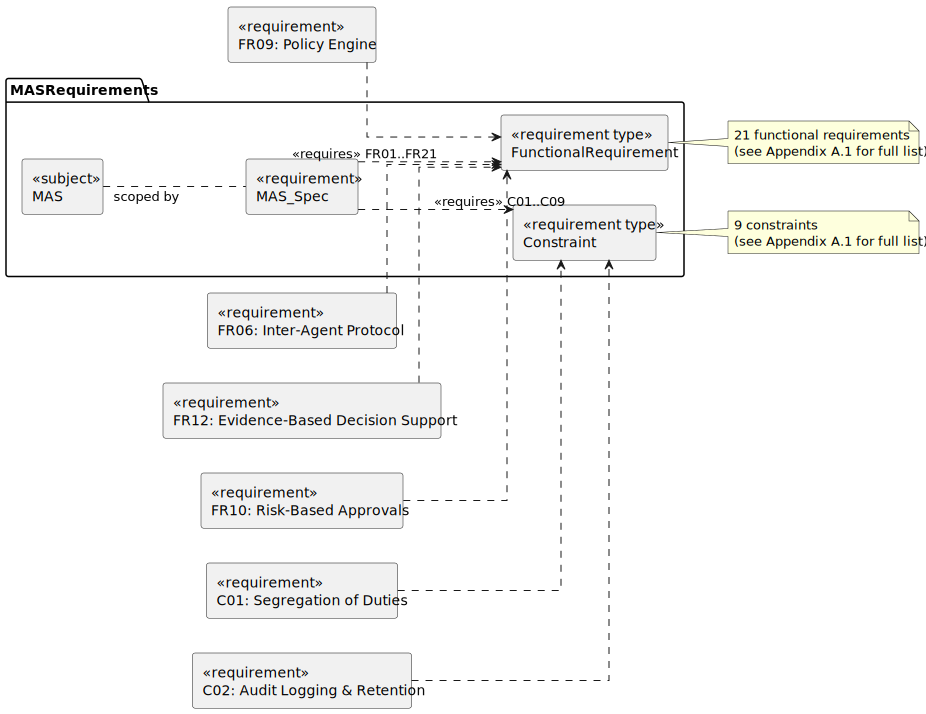
\includegraphics[width=.95\linewidth]{ressources/MAS/diagrams/fig-model-based-representation.svg}
  \caption{Model-based representation of the requirement set (subject, requirement types, consolidated group).}~\label{fig:req-model}
\end{figure}


\section{Architecture Modeling}\label{sec:mod-mas}
This section presents a general, industry-agnostic design that balances agent autonomy with governance, observability, and integration. The architecture is intentionally simple: a central orchestrator coordinates a small set of specialized agents and vetted tools; complex patterns (e.g., multi-tier supervisor trees or free-for-all peer meshes) are avoided to preserve transparency and debuggability~\parencite{langchain_multi_agents, cognition_dont_build}.

\subsection{Architecture Overview}\label{sec:arch-overview}
To keep the design industry-agnostic, the integration layer is bound to \emph{open} interfaces: \emph{Model Context Protocol (MCP)} \parencite{anthropic_mcp} standardizes agent-tool/data access via schema-driven servers/clients, while \emph{Agent-to-Agent (A2A)} \parencite{google_a2a} standardizes secure inter-agent discovery and messaging across runtimes. MCP handles agent $\leftrightarrow$ tool; A2A handles agent $\leftrightarrow$ agent—preserving portability without giving up centralized orchestration.

\begin{table}[H]
  \centering
  \small
  \begin{tabular}{p{2cm} p{5.4cm} p{5.8cm}}
    \toprule
    \textsc{Interface} & \textsc{Primary responsibility} & \textsc{Why here} \\
    \midrule
    MCP & Agent $\leftrightarrow$ Tool/Data contracts (capabilities, schemas, auth) & Uniform adapters across SaaS/on\-prem; reduces glue code; enforces I/O validation (\textsc{FR-18..21; C-08, C-09}). \\
    A2A & Agent $\leftrightarrow$ Agent messaging, discovery, long-running tasks & Vendor-neutral multi-agent collaboration across teams/orgs; complements MCP (\textsc{FR-20}). \\
    \bottomrule
  \end{tabular}
  \caption{Open protocols used by the integration layer and their scope boundaries.}
\end{table}

\noindent \textsc{design decisions} \quad A central supervisor with agents-as-tools pattern was adopted: the orchestrator invokes specialists as function/tool calls and merges results, rather than letting agents freely call one another~\parencite{langchain_multi_agents}. This yields predictable control flow and clearer accountability~\parencite{cognition_dont_build} (satisfies \textsc{C-06}, supports \textsc{FR-04, FR-08, FR-14, FR-17}).

\begin{itemize}
  \item \textsc{prompting and tool use} \quad Agents follow a \emph{reason+act} loop (ReAct): interleaving lightweight reasoning with tool calls and state updates, which improves faithfulness and reduces ungrounded steps in complex tasks~\parencite{yaoReAct2023}. Tool exposure is \emph{scoped per role} (\enquote{tool loadouts}) to minimize cognitive overhead and context bloat (\textsc{FR-19; C-09})~\parencite{breunig_context_fail,breunig_fix_context}. Prompt/context was treated as a constrained resource. The orchestrator curates per-step, minimal context; older details are summarized or offloaded to external memory; retrieval is used for relevance~\parencite{breunig_context_fail,breunig_fix_context} (supports \textsc{FR-12, FR-14, FR-15; C-07}).
  \item \textsc{coordination model} \quad Orchestrator-mediated hand-offs with explicit task payloads and expected outputs (\emph{handoff contracts}) ensure shared understanding and avoid agent conflict (\textsc{FR-06, FR-08}). Only key outcomes are published to a global scratchpad; low-level traces remain local unless needed (\textsc{FR-15; C-07})~\parencite{cognition_dont_build,langchain_multi_agents}.
  \item \textsc{parallelization} \quad Breadth-first tasks (e.g., multiple independent lookups) may run in parallel; generation tasks (long-form writing/code) remain serial or are merged under Orchestrator/Reviewer control to prevent incoherence~\parencite{langchain_multi_agents,cognition_dont_build}. The orchestrator enforces per-tool concurrency caps and rate-limit-aware backoff (jittered retries) to avoid API storms; merge operations use deterministic ordering (e.g., timestamp/key sort) and a reviewer-gated reconcile-before-write for generative outputs (\textsc{FR-04, FR-08, FR-15}).
  \item \textsc{exception handling} \quad Deviation detection $\rightarrow$ route to \emph{Exception Subprocess} (fallback tools, re-prompt, human escalation) $\rightarrow$ resume or terminate (\textsc{FR-04, FR-05, FR-07}).
\end{itemize}

\begin{table}[H]
  \centering
  \small
  \begin{tabular}{p{3.2cm} p{5cm} p{5cm}}
    \toprule
    \textsc{Pattern} & \textsc{Why/When} & \textsc{Trade-offs} \\
    \midrule
    \rowcolor{gray!13} Central orchestrator, agents-as-tools & default for clarity, traceability, testability. & Single coordination point; easiest to govern/observe. \\
    Decentralized mesh & Only for highly exploratory, research-heavy tasks. & Complex coordination, harder to debug. \\
    Hierarchical supervisors & For very large, multi-team workflows. & Adds layers and latency, out of scope for simplicity. \\
    \bottomrule
  \end{tabular}
  \caption{Chosen pattern (in gray) vs.~alternatives and scope boundaries.}
\end{table}

\noindent \textsc{integration (industry-agnostic)}
\begin{itemize}
  \item \textsc{tool adapters} with contracts/schemas, timeouts/retries/idempotency (\textsc{FR-19, FR-21; C-08, C-09}).
  \item \textsc{open connectors (MCP)} Standardize agent access to tools/data via MCP servers/clients (capabilities, JSON schemas, auth), avoiding bespoke adapters and easing on-prem + cloud integration~\parencite{anthropic_mcp} (\textsc{FR-18..21; C-05, C-08, C-09}).
  \item \textsc{agent interoperability (A2A)} Use A2A for secure agent discovery, messaging, long-running tasks, and cross-org coordination over web standards\ \parencite{google_a2a} (\textsc{FR-20}). External partners' agents become callable \emph{as if} tools—without breaking the orchestrator pattern.
\end{itemize}

\noindent \textsc{context management} \quad Right-sized prompts; retrieve-then-read; periodic summarization; external scratchpad for verbose/intermediate artifacts~\parencite{breunig_context_fail,breunig_fix_context} (supports \textsc{FR-12, FR-14, FR-15; C-07}).

\noindent \textsc{failure modes to avoid} \quad Very long prompts and indiscriminate context sharing degrade reliability (\enquote{context is not free}); prefer retrieval, summarization, and offloaded scratchpads to keep step-specific context tight~\parencite{breunig_context_fail,breunig_fix_context}.


\textsc{top-level structure} \quad The system comprises five logical layers (Fig.~\ref{fig:arch-overview}) each of which maps the primary requirement ownership; several requirements (e.g., \textsc{FR-04, FR-07, FR-10}) are cross-cutting and also appear in \textsc{design decisions} and \textsc{governance/integration}. Because progress in agentic AI is recent and evolving, the literature review establishes the broader scholarly and technical context, while this design section proritizes primary sources (official specifications and technical reports); practitioner posts are cited only to illustrate engineering trade-offs, not as authoritative evidence.

\begin{enumerate}
  \item \textsc{interaction layer} (user/client, human-in-the-loop checkpoints) --- entry point, human-machine coordination surfaces, and approval/escalation gates (\textsc{FR-03, FR-05, FR-10}).
  \item \textsc{orchestration layer} (orchestrator agent) --- decomposes tasks, sequences steps, performs policy checks; manages parameterized subprocesses and exception routing (\textsc{FR-01, FR-02, FR-04, FR-09, FR-10; C-04, C-06}).
  \item \textsc{agent layer} (specialists) --- narrow-scope agents such as researcher, analyst, reviewer/verifier, writer (\textsc{FR-06, FR-08, FR-12..14}).
  \item \textsc{tool/integration layer} --- adapters to enterprise systems via standard connectors; validates tool outputs and supports recovery/fallbacks (\textsc{FR-07, FR-18..21; C-05, C-08, C-09}).
  \item \textsc{operations and governance layer} --- logging, tracing, dashboards, replay, compliance mapping and drift checks, policy store (\textsc{FR-11, FR-15..17; C-01, C-02, C-03, C-07}).
\end{enumerate}

\begin{figure}[H]
  \centering
  \fbox{\parbox{0.92\linewidth}{
    \small \textbf{Figure placeholder (to be modeled in SysML v2)}.
    Show: User $\rightarrow$ Orchestrator $\rightarrow$ {Researcher, Analyst, Reviewer, Writer} $\rightarrow$ Tool Adapters (\textbf{MCP} servers, APIs, RAG); optional \textbf{A2A} links to external agents.
  }}
  \caption{High-level architecture (layers and main interactions).}~\label{fig:arch-overview}
\end{figure}

\textsc{roles and responsibilities}
\begin{itemize}
  \item \textsc{orchestrator} --- plans, delegates, validates, and gates risky actions; owns workflow state and shared scratchpad (\textsc{FR-01, FR-04, FR-09..11, FR-15}).
  \item \textsc{researcher} --- retrieves evidence using RAG/tools; writes salient findings to shared state (\textsc{FR-12, FR-18..21}).
  \item \textsc{analyst} --- transforms evidence (calculations, checks, comparisons); flags uncertainty and triggers escalation if needed (\textsc{FR-07, FR-12, FR-10}).
  \item \textsc{reviewer/verifier} --- critiques outputs against rules and policies; requests fixes; records rationale (\textsc{FR-13, FR-14, FR-11}).
  \item \textsc{writer} --- synthesizes final artifacts to required format; applies review feedback; preserves decision trace (\textsc{FR-14}).
\end{itemize}

Because MCP \parencite{anthropic_mcp} and A2A \parencite{google_a2a} are living industry protocols, core properties are documented primarily in official announcements/specs and arXiv technical reports; I triangulate these with emerging analyses. They are included here (design section) because they determine interface contracts and runtime behavior, not just background theory. Where possible, I cite primary protocol docs and recent surveys to mitigate gray-literature risks.

\subsection{Governance and Observability}\label{sec:gov-obs}
\textsc{governance (policy-first)} \quad A decoupled \emph{policy engine} validates proposed actions before execution (allow/deny/escalate), with rules that reference risk thresholds, data sensitivity, or regulatory constraints (\textsc{FR-09..11; C-01..03}). High-impact actions pause at \emph{approval gates} (human-in-the-loop) with resumable state\ \parencite{langgraph_hil} (\textsc{FR-10}).

\noindent \textsc{security touchpoints} \quad Protocol-level controls complement the policy engine: (i) \emph{A2A} supplies authenticated agent identity, authorization, and scoped message exchange for cross-runtime collaboration; (ii) \emph{MCP} enforces schema-validated I/O, capability-scoped tool permissions, and externalized secrets (no secrets in prompts); (iii) least-privilege credentials and per-adapter allowlists bind high-impact actions. These guardrails integrate with approval gates and audit trails (\textsc{FR-09..11, FR-15..17; C-01..C-03, C-05})~\parencite{google_a2a,anthropic_mcp}.

\noindent \textsc{threats and limitations} \quad Known risks include prompt/tool injection and data exfiltration via adapters; agent impersonation or message tampering in cross-runtime links; schema drift and capability misalignment between agent intent and MCP servers; and evaluation brittleness for multi-agent coordination. We mitigate via input sanitization, capability allowlists, signed agent identities, per-adapter least-privilege, and replayable traces; residual risk remains and is monitored operationally.

\noindent \textsc{observability} \quad Agents and the orchestrator emit structured events (prompts, tool calls/results, decisions, state changes) (\textsc{FR-15}). Operators get dashboards and alerts for anomalies; the recorded trace enables audits and deterministic replay (\textsc{FR-16, FR-17}), while concise decision rationales are persisted for accountability (\textsc{FR-14}). This trace (prompts, tool I/O, decisions) is the basis for audits and regression evaluation, and can be replayed deterministically (\textsc{FR-16, FR-17})~\parencite{langchain_multi_agents}.

\subsection{Architecture Model}

\section{Discussion: Applicability Criteria}\label{sec:discussion}

\section{Conclusion}\label{sec:conclussion}
%Future work should extend this conceptual design into practical evaluation and implementation. In particular, empirical validation of the architecture in industry settings, tool-supported instantiation in SysML, and comparative studies against traditional workflow automation would provide valuable evidence of its applicability and impact. Further, integrating additional agentic AI capabilities such as autonomous negotiation or explainability could enhance both usability and compliance assurance.
% Bibliography
\clearpage
\phantomsection\
\addcontentsline{toc}{section}{References}
\markboth{References}{References}
\section*{References}
\printbibliography[heading=none]

% --- Appendix ---
\clearpage
\appendix
\refstepcounter{section}
\setcounter{subsection}{0}
\phantomsection~\addcontentsline{toc}{section}{Appendix}
\markboth{Appendix}{Appendix}
\begin{center}\huge\bfseries Appendix\end{center}

\refstepcounter{subsection}
\subsection*{\thesection.\arabic{subsection}: Requirements List}\label{app:req-list}
\noindent \textsc{functional requirements} \\
\begin{footnotesize}
\noindent \textsc{FR-01 process orchestration engine} --- The system shall execute workflow models by dispatching tasks to human or software actors according to model control flow and business rules. \\
\noindent \textsc{FR-02 parameterized subprocesses} --- The system shall support parameterized subprocesses and rules so behavioral variants can be expressed without altering the underlying process structure. \\
\noindent \textsc{FR-03 human-machine task orchestration} --- The system shall coordinate both human and automated tasks within the same orchestrated process model. \\
\noindent \textsc{FR-04 exception detection and routing} --- The system shall detect deviations from the nominal process and route cases to defined exception subprocesses. \\
\noindent \textsc{FR-05 escalation to human authority} --- The system shall escalate unresolved or unmodeled exceptions to designated human roles with clear ownership. \\
\noindent \textsc{FR-06 inter-agent communication protocol} --- The system shall specify message formats and interaction rules for agent collaboration (e.g., direct messaging or shared memory; event-bus/blackboard where asynchronous exchange is required).\\
\noindent \textsc{FR-07 tool failure handling in exceptions} --- The system shall validate tool/API outputs and trigger defined recovery or fallback steps when invocations fail.\\
\noindent \textsc{FR-08 conflict resolution} --- The system shall provide mechanisms for agents to resolve task or decision conflicts (e.g., delegation to a planner, negotiation, or voting).\\
\noindent \textsc{FR-09 policy engine} --- The system shall provide a decoupled policy evaluation component that can validate, veto, or redirect workflow executions and agent actions at runtime. \\
\noindent \textsc{FR-10 risk-based approvals and escalation} --- The system shall require human approval and/or escalation for actions or decisions exceeding defined risk or impact thresholds. \\
\noindent \textsc{FR-11 compliance mapping and drift checks} --- The system shall map actions and policies to applicable regulations or internal rules and perform runtime checks to detect and block compliance drift. \\
\noindent \textsc{FR-12 evidence-based decision support} --- The system shall aggregate relevant data at decision points to support evidence-based choices and reduce errors. \\
\noindent \textsc{FR-13 rule-enforced decision points} --- The system shall enforce business rules and role responsibilities at decision points to ensure consistent, auditable outcomes. \\
\noindent \textsc{FR-14 decision trace and rationale} --- The system shall persist a human-readable decision trace for automated or assisted decisions, including inputs, tool/API calls and results, and concise rationale summaries. \\
\noindent \textsc{FR-15 event logging pipeline} --- The system shall instrument the workflow engine and agents to emit structured, timestamped events for key actions (e.g., prompts, tool/API invocations and results, plan/decision commits, and state changes). \\
\noindent \textsc{FR-16 dashboards and alerts} --- The system shall provide real-time dashboards and alerting for observability metrics (e.g., execution latency, error/anomaly rates, blocked actions). \\
\noindent \textsc{FR-17 replay for post-hoc analysis} --- The system shall support reconstruction and replay of workflow and agent interactions from logged events to enable root-cause analysis and explanation of outcomes. \\
\noindent \textsc{FR-18 integration connectors} --- The system shall provide connectors to integrate heterogeneous applications and data sources required by the workflows. \\
\noindent \textsc{FR-19 agent tool adapters} --- The system shall expose a uniform adapter interface for agents and workflows to invoke external tools, APIs, databases, or RPA scripts. \\
\noindent \textsc{FR-20 inter-organizational interoperability} --- The system shall support protocol and interface interoperability suitable for cross-organizational workflows. \\
\noindent \textsc{FR-21 data transformation layer} --- The system shall provide mapping and transformation capabilities to reconcile data across integrated systems. \\
\end{footnotesize}

\noindent \textsc{constraints} \\
\begin{footnotesize}
\noindent \textsc{C-01 segregation of duties} --- The system shall enforce role-based access control and segregation of duties for configuration changes and sensitive actions. \\
\noindent \textsc{C-02 audit logging and retention} --- The system shall produce tamper-evident audit trails of agent actions, policy decisions, and configuration changes, retained according to the applicable compliance policy. \\
\noindent \textsc{C-03 bounded decision autonomy} --- The system shall constrain agent decision-making to clearly scoped authority levels aligned with organizational objectives. \\
\noindent \textsc{C-04 modular process units} --- The system shall structure workflows as modular subprocesses or services that can be reused and reconfigured without redesign. \\
\noindent \textsc{C-05 interface-based composition} --- The system shall expose clear process and service interfaces compatible with established interoperability standards to enable composition across heterogeneous systems and organizations. \\
\noindent \textsc{C-06 explicit coordination model} --- The system shall define and enforce a coordination structure (e.g., hierarchical planner–specialists or decentralized collaboration) for multi-agent work. \\
\noindent \textsc{C-07 agent status self-reporting} --- The system shall require agents to periodically self-report status and progress (e.g., current task, step outcome, next planned action) to improve runtime transparency. \\
\noindent \textsc{C-08 interface contracts and schemas} --- The system shall define input/output contracts and validate request/response schemas at adapter boundaries. \\
\noindent \textsc{C-09 invocation safeguards} --- The system shall enforce adapter-level safeguards (e.g., timeouts, retries, and idempotency keys) to limit side effects of failed or repeated tool calls.
\end{footnotesize}

\subsection*{A.2 Requirements Model}
\begin{figure}[H]
  \centering
  
\includegraphics[width=\linewidth]{ressources/MAS/diagrams/MASRequirements.pdf}\label{fig:req}
\end{figure}

\subsection*{A.3 Requirements SysML v2 Code}
\lstinputlisting[
  style=sysml,
  caption={Requirements model (MASRequirements.sysml)},
  label={lst:mas-reqs},
  numbers=left,
  inputencoding=utf8
]{./ressources/MAS/MASRequirements.sysml}

\subsection*{B.1 Architecture Model}
\begin{figure}[H]
  \centering
  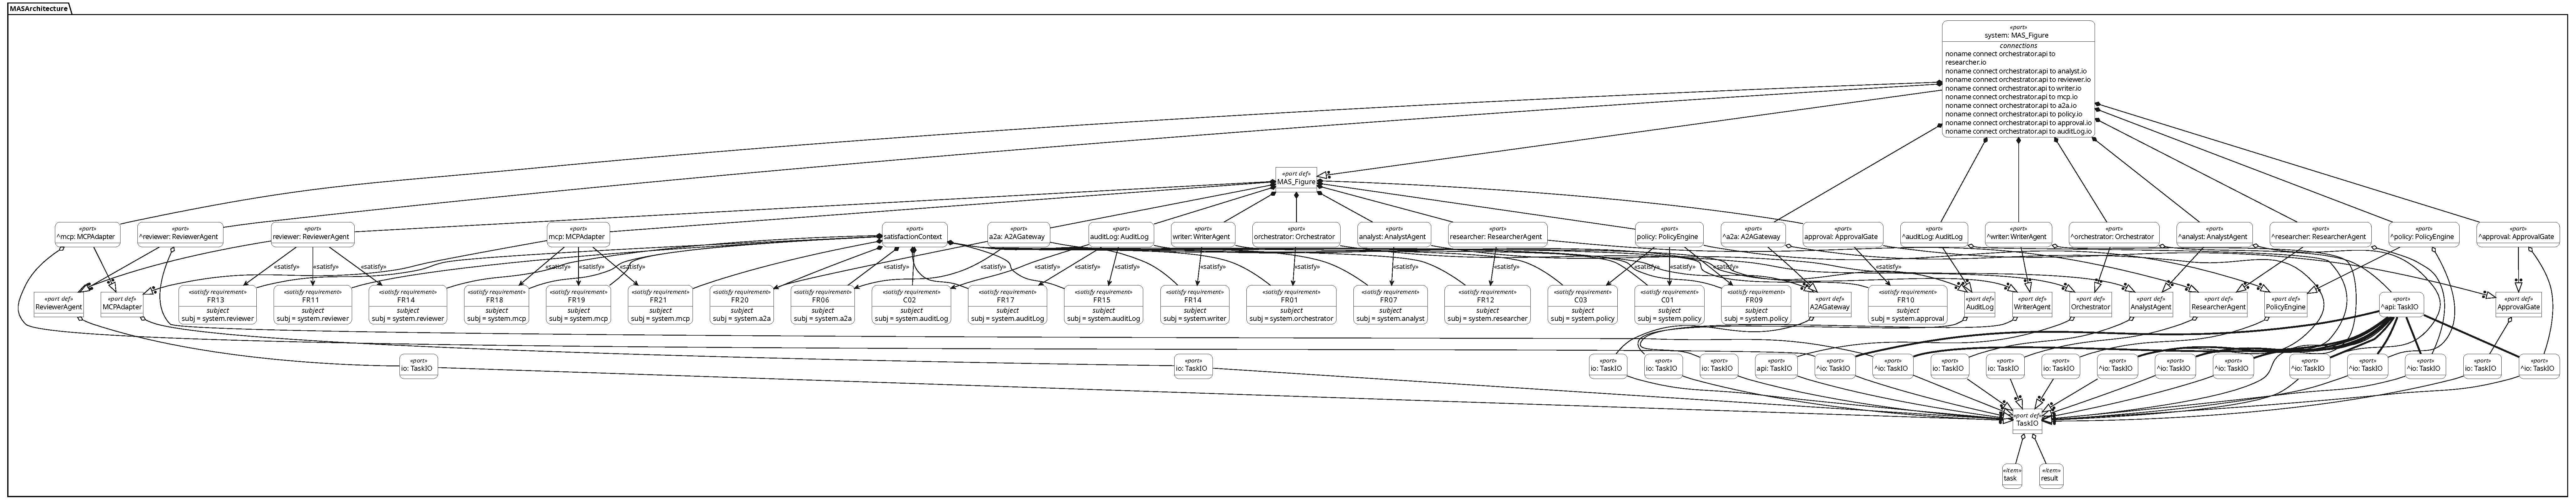
\includegraphics[width=\linewidth]{ressources/MAS/diagrams/MASArchitecture.pdf}\label{fig:arch}
\end{figure}

\subsection*{B.2 Architecture SysML v2 Code}
\lstinputlisting[
  style=sysml,
  caption={Architecture model (MASArchitecture.sysml)},
  label={lst:mas-arch},
  inputencoding=utf8
]{./ressources/MAS/MASArchitecture.sysml}

\subsection*{B.2 Architecture Figure}
\begin{figure}[H]
  \centering
  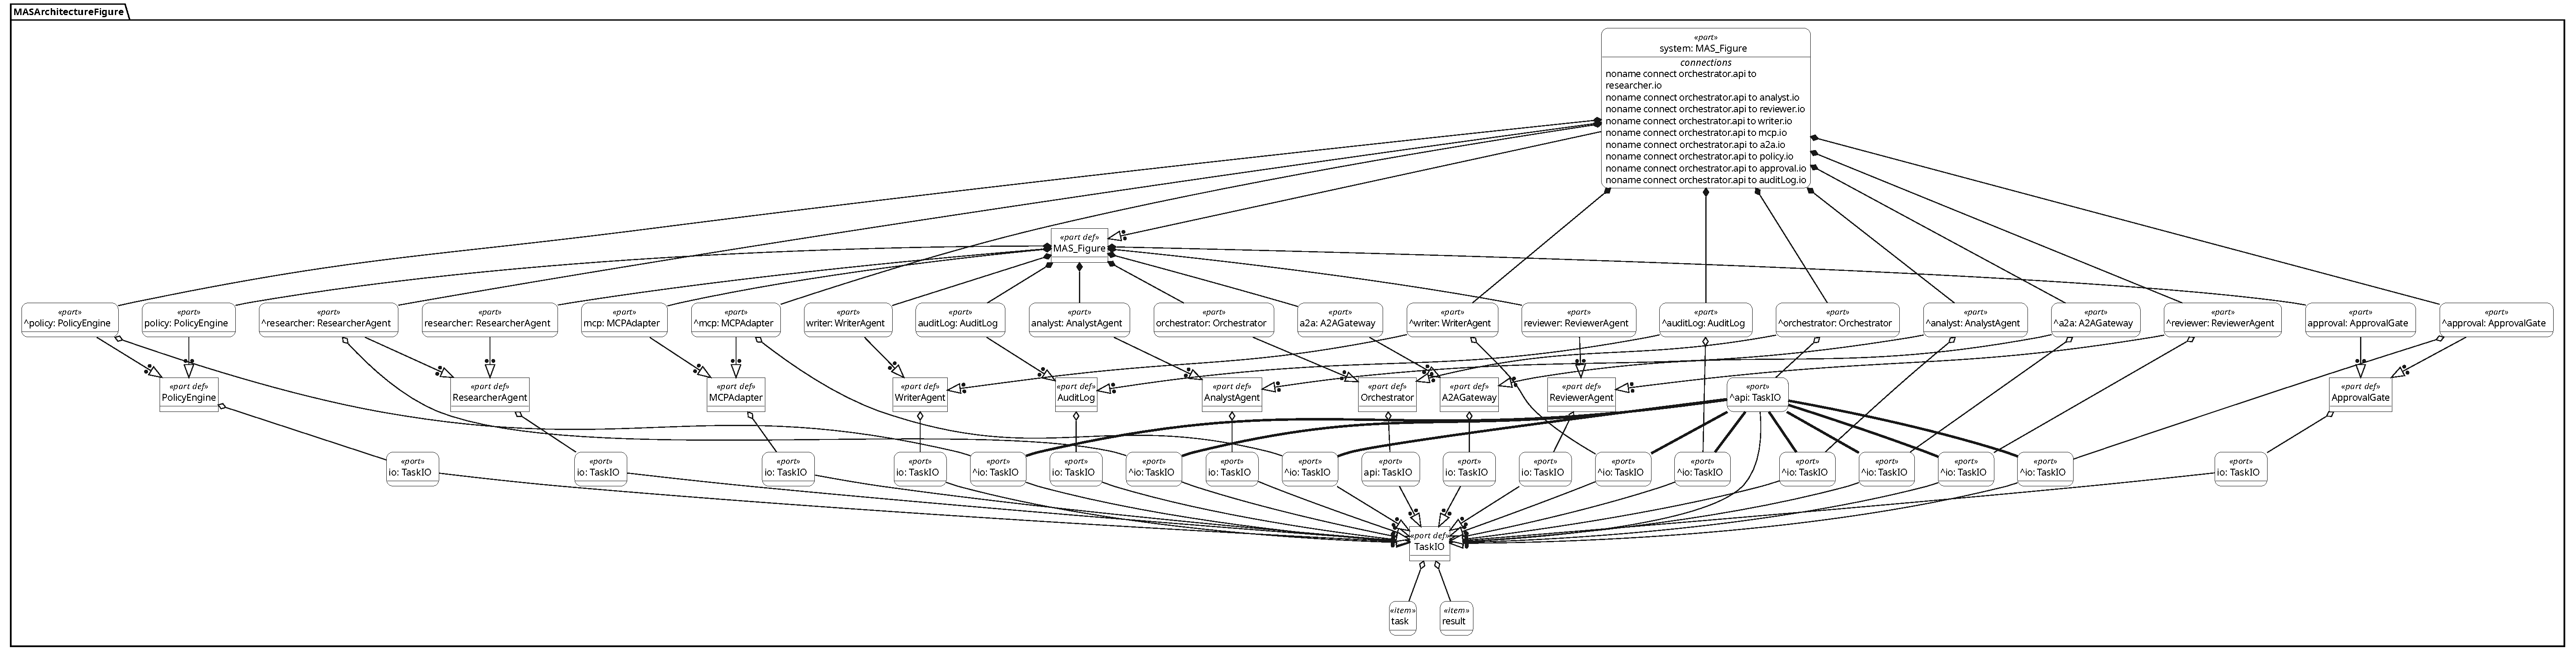
\includegraphics[width=\linewidth]{ressources/MAS/diagrams/MASArchitecture_Figure.pdf}\label{fig:arch-fig}
\end{figure}

\subsection*{B.3 Architecture Figure SysML v2 Code}
\lstinputlisting[
  style=sysml,
  caption={Architecture figure (MASArchitecture\_Figure.sysml)},
  label={lst:mas-arch-figure},
  inputencoding=utf8
]{./ressources/MAS/MASArchitecture_Figure.sysml}

\subsection*{C.1 Traceability Diagram}
\begin{figure}[H]
  \centering
  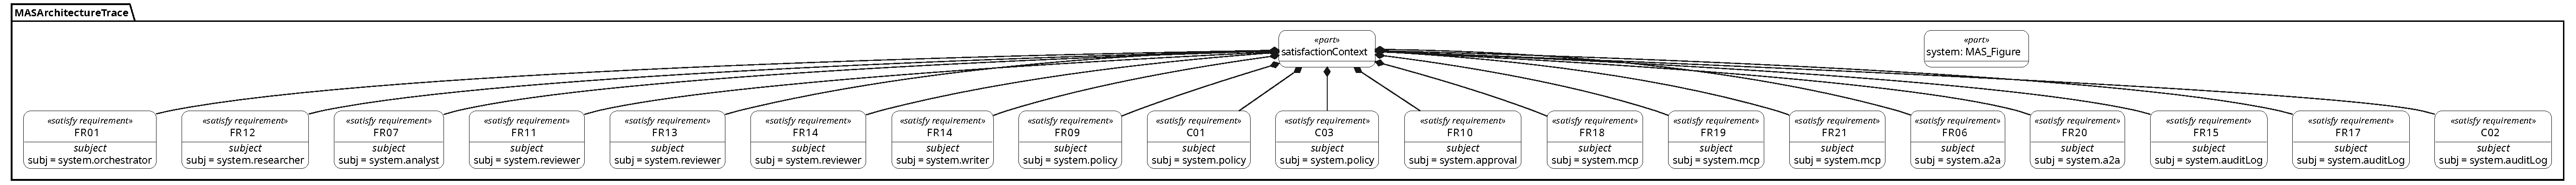
\includegraphics[width=\linewidth]{ressources/MAS/diagrams/MASArchitecture_Trace.pdf}\label{fig:trace}
\end{figure}

\subsection*{C.2 Traceability SysML v2 Code}
\lstinputlisting[
  style=sysml,
  caption={Traceability mapping (MASArchitecture\_Trace.sysml)},
  label={lst:mas-arch-trace},
  inputencoding=utf8
]{./ressources/MAS/MASArchitecture_Trace.sysml}

\subsection*{C. 3 Traceability}
\begin{figure}[H]
  \centering
  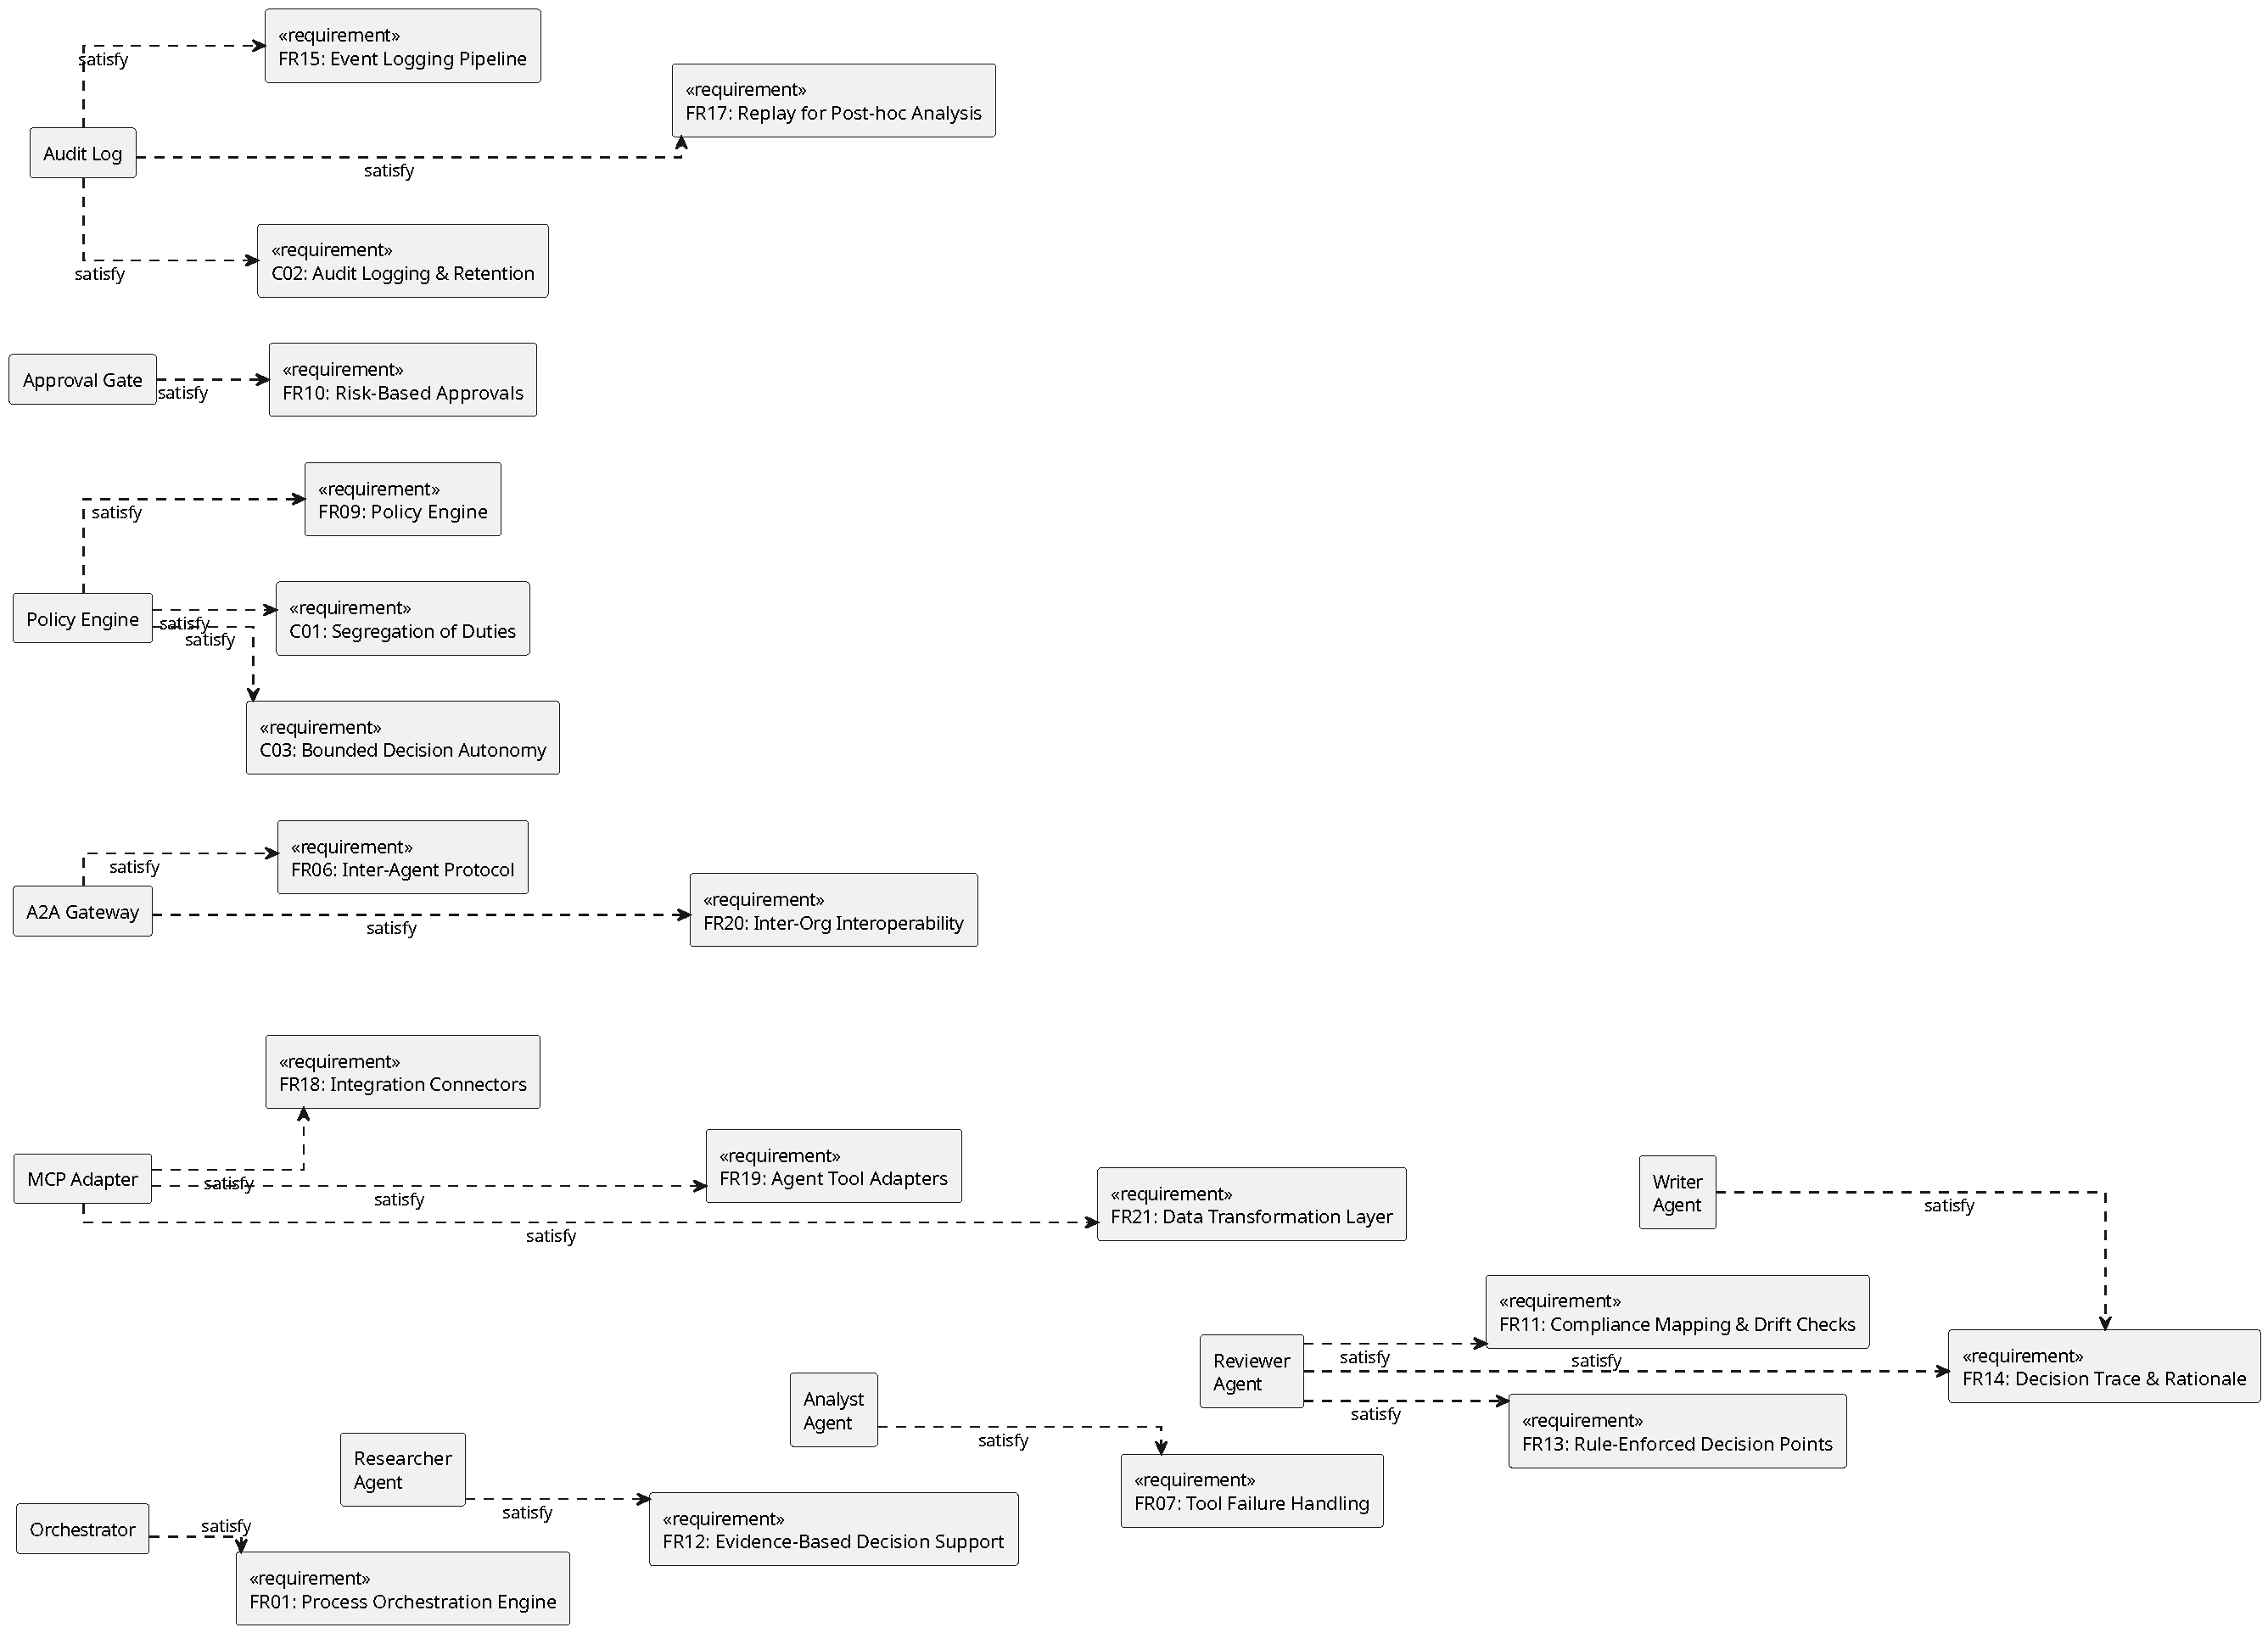
\includegraphics[width=\linewidth]{ressources/MAS/diagrams/fig-traceability.pdf}\label{fig:trace-fig}
\end{figure}

% --- NDA ---
% \clearpage
% \thispagestyle{empty}
% \begin{center}
% 	\vspace*{1cm}
% 	\Huge\textbf{Non-Disclosure Agreement}\\
% 	\vspace*{2cm}
% 	\normalsize
% 	\begin{quotation}
% 		\parbox{0.8\textwidth}{The present bachelor's thesis contains internal confidential information of the company \myCompany, \myCompanyAddress. The dissemination of the content of the work in whole or in part is strictly prohibited. No copies or transcripts, including digital forms, cane made. Exceptions require the written approval of the company \myCompany.}
% 	\end{quotation}
% 	\vspace*{1cm}
% 	\begin{quotation}
% 		\parbox{0.8\textwidth}{
% 		\begin{tabularx}{0.78\textwidth}{l@{\extracolsep\fill}l}
%             \small \myLocation, \today \\
% 	        \rule{6cm}{0.1mm}&\rule{4cm}{0.1mm}\\
% 			Place, Date&Signature
% 		\end{tabularx}}
% 	\end{quotation}
% \end{center}
% \newpage

% --- AI Declaration ---                               
\end{document}